\chapter{Teoretické porovnanie API tokenov}

\label{kap:teoreticke} % id kapitoly pre prikaz ref

V tejto kapitole porovnáme rôzne vlastnosti a parametre konkrétnych tokenov podľa informácií získaných z ich dokumentácií a iných zdrojov. Niektoré dáta sme už zhrnuli v kapitole \ref{kap:typy} a preto ich tu nespomíname alebo nevysvetľujeme. Pri jednotlivých parametroch vysvetlíme ich význam a teda aj dôležitosť pri porovnávaní tokenov. Porovnávať budeme všetky štruktúrované tokeny popísané v kapitole \ref{kap:typy} a nepriehľadný formát tokenu popísaný v~podkapitole \ref{sec:opaque}. Pre jednoduchosť budeme pod pojmom nepriehľadný token myslieť náhodný reťazec s podpisom vo forme hešovaného autentifikačného kódu. 

\begin{table}[H]
  \begin{center}
    \caption{Teoretické porovnanie tokenov}
    \label{tab:porovnanie} % create a label for the table, after caption
    
    \resizebox{\columnwidth}{!}{%
    \begin{tabular}{lccccccc}
      \hline
      Vlastnosť & Nepriehľadný & JWT & PASETO & Fernet & Branca & Macaroons & Biscuits\\
      \hline
      Počet kryptografických funkcií & 1 & 30 & 6 & 1 & 1 & 1 & 1\\
      Určenie podpisového algoritmu z tokenu & $\varoslash$ & \CIRCLE & \CIRCLE & \Circle & \Circle & \Circle & \Circle \\
      Náchylnosť na útok pomýlením algortimu & $\varoslash$ & \CIRCLE & \LEFTcircle & \Circle & \Circle & \Circle & \Circle \\
      Riešenie problému odvolania & \CIRCLE & \Circle & \Circle & \Circle & \Circle & \LEFTcircle & \LEFTcircle \\
      Náchylnosť na útok opakovaním & $\varoslash$ & \CIRCLE & \CIRCLE & \CIRCLE & \CIRCLE & \LEFTcircle & \LEFTcircle \\
      Ochrana dôvernosti & $\varoslash$ & \LEFTcircle & \LEFTcircle & \CIRCLE & \CIRCLE & \Circle & \Circle \\
      Overenie autentickosti a integrity hocikým & \Circle & \LEFTcircle & \CIRCLE & \CIRCLE & \CIRCLE & \CIRCLE & \CIRCLE \\
      Zoslabenie tokenu hocikým & $\varoslash$ & $\varoslash$ & $\varoslash$ & $\varoslash$ & $\varoslash$ & \CIRCLE & \CIRCLE \\
      Autorizačná schéma v tokene & $\varoslash$ & \LEFTcircle & \LEFTcircle & \LEFTcircle & \LEFTcircle & \CIRCLE & \CIRCLE \\
      Bezstavová validácia & $\varoslash$ & \CIRCLE & \CIRCLE & \CIRCLE & \CIRCLE & \CIRCLE & \CIRCLE \\
      Štandardná validácia & $\varoslash$ & \CIRCLE & \CIRCLE & \Circle & \Circle & \LEFTcircle & \CIRCLE \\
      Popularita & $\varoslash$ & \CIRCLE & \LEFTcircle & \LEFTcircle & \Circle & \LEFTcircle & \Circle \\
      \hline
    \end{tabular}%
    }
  \end{center}
\end{table}

Kapitola je štruktúrovaná podľa porovnávaných vlastností a jej výsledkom je tabuľka \ref{tab:porovnanie} zhrňujúca závery porovnania. Tabuľku uvádzame na začiatku kapitoly, aby si čitateľ mohol utvoriť istý prehľad o porovnávaných vlastnostiach. V tabuľke používame symboly \CIRCLE, \LEFTcircle ~a \Circle ~pre vyjadrenie stupňovitosti istej kvality tokenu. Symbol \CIRCLE ~znamená, že vlastnosť je pre daný token typická, častá alebo dôležitá. Symbol \Circle ~vyjadruje presný opak a symbol \LEFTcircle ~niečo medzi tým. Symbol $\varoslash$ ~znamená, že vlastnosť sa nedá pre daný token posúdiť alebo z nejakého dôvodu nemá zmysel o nej uvažovať a~porovnávať ju. Na začiatku každej podkapitoly uvedieme časť tabuľky, ktorá sa venuje vlastnostiam porovnávaným v danej podkapitole.

\section{Bezpečnosť}

V rámci porovnávania bezpečnosti tokenov nebudeme detailne rozoberať bezpečnosť jednotlivých kryptografických funkcií. Detaily ohľadom týchto funkcií je možné nájsť v~ich citovaných dokumentáciách. Všetky tokeny ponúkajú možnosť použiť kryptografické funkcie, ktoré sú všeobecne považované za bezpečné. Zhrnutie výsledkov porovnania bezpečnosti tokenov je možné nájsť v tabuľke \ref{tab:bezpecnost}.

\begin{table}[H]
  \begin{center}
    \caption{Bezpečnosť tokenov}(vybrané riadky tabuľky \ref{tab:porovnanie} relevantné pre bezpečnosť)
    \label{tab:bezpecnost} % create a label for the table, after caption

    \resizebox{\columnwidth}{!}{%
    \begin{tabular}{lccccccc}
      \hline
      Vlastnosť & Nepriehľadný & JWT & PASETO & Fernet & Branca & Macaroons & Biscuits\\
      \hline
      Počet kryptografických funkcií & 1 & 30 & 6 & 1 & 1 & 1 & 1\\
      Určenie podpisového algoritmu z tokenu & $\varoslash$ & \CIRCLE & \CIRCLE & \Circle & \Circle & \Circle & \Circle \\
      Náchylnosť na útok pomýlením algortimu & $\varoslash$ & \CIRCLE & \LEFTcircle & \Circle & \Circle & \Circle & \Circle \\
      Riešenie problému odvolania & \CIRCLE & \Circle & \Circle & \Circle & \Circle & \LEFTcircle & \LEFTcircle \\
      Náchylnosť na útok opakovaním & $\varoslash$ & \CIRCLE & \CIRCLE & \CIRCLE & \CIRCLE & \LEFTcircle & \LEFTcircle \\
      Ochrana dôvernosti & $\varoslash$ & \LEFTcircle & \LEFTcircle & \CIRCLE & \CIRCLE & \Circle & \Circle \\
      Overenie autentickosti a integrity hocikým & \Circle & \LEFTcircle & \CIRCLE & \CIRCLE & \CIRCLE & \CIRCLE & \CIRCLE \\
      \hline
    \end{tabular}%
    }
  \end{center}
\end{table}

Zameriame sa na porovnanie kryptografických primitív a z nich vyplývajúcich bezpečnostných kvalít a na náchylnosť na zraniteľnosti vyplývajúce zo špecifikácie tokenov. Konkrétne rozoberieme tri bezpečnostné problémy:


\begin{itemize}
  \item Útok pomýlením algoritmu (angl. algorithm confusion attack) -- útočník donúti overovaciu službu použiť nesprávny algoritmus na overenie podpisu tokenu. 
  \item Útok opakovaním (angl. replay attack) -- útočník odchytí token a následne ho opakovane používa na autorizáciu vlastných požiadaviek. Tento útok je priamo spojený s hlavnou nevýhodou používania tokenov v autentifikačnej a autorizačnej schéme a to problémom odvolania (angl. revocation).
  \item Problém odvolania -- problém odvolania spočíva v schopnosti služby zneplatniť vydané tokeny. Napríklad po odhlásení používateľa alebo po zistení, že token bol zneužitý.
\end{itemize}


\subsection{Kryptografické primitíva}

Pri tokenoch rozoznávame tri kryptografické primitíva a to digitálne podpisy využívajúce asymetrické šifrovanie, symetrické šifrovanie a hešovanie s kľúčom. Výstupom hešovania s kľúčom je hešovaný autentifikačný kód.

Symetrické šifrovanie sa v rámci nami porovnávaných tokenov využíva na šifrovanie obsahu tokenu a teda na ochranu dôvernosti informácií uložených v tokene. Digitálny podpis a hešovanie s kľúčom zaručujú ochranu autenticity a integrity tokenu. Rozdiel v použití digitálneho podpisu a hešovania s kľúčom je v tom, že v prípade digitálneho podpisu ide o asymetrické šifrovanie, teda  podpis vie overiť ľubovoľná entita, ktorá pozná verejný kľúč tvoriaci dvojicu so súkromným kľúčom, ktorým bol token podpísaný. Takýto verejný kľúč je zväčša verejne dostupný a vie ho získať ľubovoľná entita. V prípade hešovania s kľúčom ide o symetrickú kryptografiu, pravosť hešovaného autentifikačného tokenu vie overiť len entita, ktorá pozná tajný kľúč, ktorým bol token zahešovaný, čo je často len entita, ktorá token vytvorila.

Výhodou digitálneho podpisu teda je, že autenticitu a integritu tokenu môže overiť ľubovoľná entita. Výhodou hešovania s kľúčom je, že je rýchlejšie pri generovaní kľúča a generovaní aj overovaní podpisu ako algoritmy pre digitálne podpisy, aj keď v prípade niektorých algoritmov nad eliptickými krivkami je rýchlosť porovnateľná \cite{hmac_perf}. Pri porovnaní iba algoritmov definovaných v JWA \cite{hmac_jwt_perf} je hešovanie s kľúčom vždy rýchlejšie.

V prípade JWT si môžeme vybrať, či budeme používať digitálny podpis alebo hešovanie s kľúčom pomocou nastavenia oprávnenia \textit{alg} v hlavičke na požadovanú hodnotu. Všetky možnosti hodnôt oprávnenia \textit{alg} definuje  JWA \cite{jwa_rfc}. Štandard ponúka aj možnosť \textit{alg=none}, v tomto prípade nezaručuje JWT žiadne bezpečnostné kvality a je to jedna zo známych zraniteľností \cite{jwt_vul} JWT. Ak služba akceptuje aj JWT s \textit{alg=none} ako platné tokeny, útočník jednoducho zamení hodnotu \textit{alg='čokoľvek'} na \textit{alg=none}, odstráni podpis z tokenu a môže ľubovoľne zmeniť token, napríklad si zvýši autorizačné práva. Bezpečné implementácie JWT, by nikdy nemali tokeny s \textit{alg=none} považovať za platné.

PASETO využíva v prípade lokálneho využitia hešovanie s kľúčom a v prípade verejného využitia digitálny podpis. Fernet, Branca a Macaroons využívajú hešovanie s kľúčom a~Biscuits využíva digitálny podpis. Nepriehľadný token sme pre potreby tejto kapitoly definovali s použitím hešovania s kľúčom.

Symetrické šifrovanie a z neho vyplývajúcu ochranu dôvernosti umožňujú tokeny JWT, konkrétne vo forme JWE, PASETO s lokálnym využitím, Fernet a Branca. Biscuits a Macaroons neposkytujú žiadnu ochranu dôvernosti. Nepriehľadný token tiež neposkytuje ochranu dôvernosti v rámci tokenu, no z definície nenesie žiadnu informáciu a všetky dôverné údaje sú uložené na strane servera a asociované s tokenom. Teda na strane klienta nie je dôvernosť čoho chrániť.

\subsection{Útok pomýlením algoritmu}

V prípade podpisov tokeny používajú digitálne podpisy na základe asymetrického šifrovania a teda dvojicu súkromného a verejného kľúča alebo hešovanie s kľúčom, ktorý je tajný. Jediný kľúč, ku ktorému má útočník ľahký prístup je verejný kľuč (označme ho $pk$). Útok pomýlením algoritmu potom prebehne tak, že útočník podpíše token hešovacou funkciou s kľúčom, kde ako kľúč použije získaný verejný kľúč $pk$. Následne oklame overovaciu službu, aby token overila pomocou hešovacej funkcie s kľúčom, kde ako kľúč použije $pk$. Ako útočník môže oklamať overovaciu službu popíšeme neskôr v podkapitole na príklade konkrétnej zraniteľnosti JWT. Takýmto spôsobom overovacia služba potvrdí platnosť ľubovoľného tokenu, ktorý jej útočník podvrhne. Aby bol tento útok úspešný, musí overovacia služba používať digitálne podpisy ako podpis tokenu a zároveň podporovať aj vytváranie podpisu tokenu pomocou hešovania s kľúčom.

Existuje viacero spôsobov ako predchádzať útokom pomýlením algoritmu. Najspoľahlivejším spôsobom je podpora jediného kryptografického primitíva na podpis tokenu, napríklad jedine digitálny podpis alebo jedine hešovanie s kľúčom. Takto útočník jednoducho nemá ako oklamať overovaciu službu, ktorý algoritmus má použiť pri overovaní, lebo pozná len jeden. 

V prípade použitia viacerých kryptografických primitív sa dá predchádzať týmto útokom pomocou vloženia identifikátora kľúča, ktorým sa overí podpis, do tokenu. Následne pri overovaní služba zistí, ktorým algoritmom bol token podpísaný. Taktiež z~pridaného identifikátora odvodí, ktorý kľúč má použiť na overenie, ak je to verejný kľúč z dvojice kľúčov pre digitálne podpisovanie, ale zistený podpisový algoritmus z~tokenu je hešovanie s kľúčom, vyhodnotí token za neplatný. Útočník už nedokáže oklamať službu aby použila zlý algoritmus na overenie podpisu, lebo ak by sa o to pokúsil nebude sedieť identifikátor kľúča s podpisovým algoritmom. Úspešnosť tejto metódy ochrany nezávisí len od špecifikácie tokenu, ale najmä od jeho konkrétnej implementácie, pretože záleží na implementácii ako bude pracovať s identifikátorom kľúča a či vôbec vyžaduje jeho použitie.

Tokeny využívajúce jediné kryptografické primitívum sú Fernet, Branca, Biscuits a~Macaroons. Sú teda bezpečné proti útokom pomýlením algoritmu, no všetky nejakým spôsobom podporujú budúce verzionovanie tokenu, ktoré môže teoreticky priniesť aj nové kryptografické primitíva. Preto do budúcnosti môžu byť zraniteľné útokom pomýlením algoritmu, ak nebudú implementovať inú ochranu voči tomuto útoku. V~súčasnosti už Macaroons aj Biscuits vyžadujú vloženie identifikátora kľúča do tokenu v~rámci ich formátov, teda aj v prípade podpory ďalších kryptografických primitív budú bezpečné voči útokom pomýlením algoritmu.

Jediné kryptografické primitívum využíva aj nepriehľadný token, ale v tomto prípade to nie je veľmi dôležité, lebo nenesie žiadnu informáciu a všetky autorizačné údaje sú uložené v stave overovacej služby. Teda aj v prípade úspešného útoku pomýlením algoritmu, služba síce vyhodnotí podpis tokenu za platný, no ak nezodpovedá žiadnym dátam uloženým v stave služby, tak služba neautorizuje útočníkovu požiadavku, na ktorú nemá inak právo. Nepriehľadný token je teda absolútne bezpečný voči útokom pomýlením algoritmu.

Viac kryptografických primitív využívajú JWT a PASETO. Oba podporujú digitálne podpisy aj hešovanie s kľúčom na podpisovanie tokenu. V prípade JWT bol útok pomýlením algoritmu jednou zo známych zraniteľností v niektorých implementáciách \cite{jwt_vul}. Konkrétne útok prebiehal tak, že útočník si vybral službu používajúcu digitálny podpis. Získal jej verejný kľúč $pk$, vytvoril podvodný token \textit{mal\_token} a do jeho hlavičky zapísal \textit{alg=HS256} (HS256 označuje funkciu HMAC-SHA256), následne funkciou HMAC-SHA256 podpísal token s využitím $pk$ ako tajného kľúča pre funkciu. Služba, ktorá využívala zraniteľnú knižnicu a na podpisovanie iba digitálny podpis overila token zavolaním funkcie knižnice, napríklad \textit{verify(pub\_key, mal\_token)}, lebo si myslela, že overuje token podpísaný digitálnym podpisom a na jeho overenie teda treba verejný kľúč $pk$. Knižnica následne prečítala z tokenu, že má overiť podpis pomocou HMAC-SHA256 a z prvého argumentu funkcie \textit{verify}, že má pri tom využiť $pk$ ako kľúč. Toto overenie bolo samozrejme úspešné, lebo token bol naozaj podpísaný funkciou HMAC-SHA256 s kľúčom $pk$. Popísaný útok je schematicky znázornený na obrázku \ref{fig:conf_alg_attack}. V súčasnosti už tieto konkrétne implementácie zaviedli ochranu voči útoku pomýlením algoritmu (pomocou identifikátora kľúča), no nič nezaručuje, že neexistujú iné implementácie s touto zraniteľnosťou. Popísaný útok dáva útočníkovi možnosť získať ľubovoľné práva, lebo celý \textit{mal\_token} môže vytvoriť presne tak ako potrebuje. Išlo teda o veľmi nebezpečný útok.

\begin{figure}
  %vlozenie samotneho obrazku vycentrovaneho a vhodnej velkosti
  %obrazok je v subore images/session.png
  \centerline{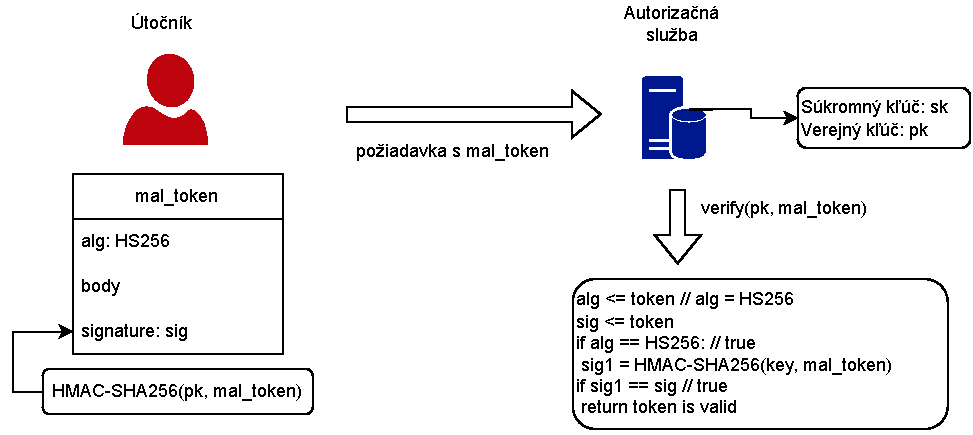
\includegraphics[width=0.8\textwidth]{images/conf_alg_attack}}
  %popis obrazku
  \caption[Útok pomýlením algortimu]{Schéma útoku pomýlením algoritmu \cite{jwt_vul}.}
  %id obrazku, pomocou ktoreho sa budeme na obrazok odvolavat
  \label{fig:conf_alg_attack}
\end{figure}

PASETO využíva verzionovanie tokenu ako prevenciu voči útoku pomýlením algoritmu. Ide o podobnú techniku ako pri vložení identifikátora kľúča do tokenu, no navyše vyžaduje kontrolu formátu kľúča. Špecifikácia PASETO \cite{paseto_git} prikazuje každej knižnici, ktorá chce implementovať PASETO, logicky rozlišovať medzi kľúčmi určenými pre rôzne podpisové funkcie. V rámci špecifikácie sa ochrane voči útoku pomýlením algoritmu venuje dedikovaný dokument \cite{alg_lucidity}. Kľúč k ľubovoľnému algoritmu musí byť vždy uložený tak, aby sa dalo jasne určiť, pre ktorý algoritmus sa má použiť. Tento cieľ sa dá dosiahnuť napríklad tak, že sa kľúč uloží v nejakej štruktúre spolu s verziou a využitím tokenu. Následne pri validácii podpisu tokenu musí prebehnúť kontrola rovnosti verzie a využitia v kľuči s verziou a využitím v tokene. Podobne ako pri JWT popísaná ochrana bude úspešná len v prípade, že ju knižnice implementujúce PASETO budú využívať. Výhodou PASETO je, že sa ochrana vyžaduje v špecifikácii, teda každá knižnica, ktorá chce úspešne implementovať špecifikáciu PASETO ju musí implementovať. V prípade JWT, štandard \cite{jwt_rfc} nevyžaduje využitie identifikátora kľúča.

S útokom pomýlením algoritmu súvisí aj celkový počet podporovaných podpisových a šifrovacích algoritmov. V tomto prípade ide skôr o problém pomýlenia algoritmu. Kryptografické algoritmy majú podobné názvy, ľahko sa teda môže stať, že sa programátor pri ich výbere pomýli a napríklad pri generovaní a validácii tokenu použije rôzny algoritmus. Toto nevedie priamo k zraniteľnostiam, no môže mať za následok nepredvídateľné správanie systému. Principiálne ide o útok pomýlením algoritmu pri každej validácii tokenu, lebo token sa nevaliduje očakávaným algoritmom. Pre útočníka je však ťažšie (potenciálne nemožné) vyrobiť falošný platný token.

Nepriehľadný token, Fernet, Branca, Macaroons aj Biscuits používajú len jednu kombináciu podpisového a šifrovacieho algoritmu. PASETO však vo všetkých potenciálnych kombináciách verzie a využitia používa dokopy 6 algoritmov. JWT dokonca až 30.

\subsection{Útok opakovaním a problém odvolania}

\label{sec:replay} % id kapitoly pre prikaz ref

Útok opakovaním a problém odvodenia sú úzko späté pojmy. Konkrétne, riešenie problému odvolania je čiastočnou ochranou voči útoku opakovaním. Ak by služba vedela okamžite zneplatniť ľubovoľný ňou vydaný token, útok opakovaním by mohla ihneď po odhalení zastaviť zneplatnením tokenov využitých pri útoku. Úplne predísť útoku opakovaním je pri využívaní nositeľských tokenov na autorizáciu nemožné. Z definície nositeľský token autorizuje požiadavku, ktorú sprevádza, ak je sám platný. Teda ak ho dokáže útočník získať a použiť v správnom kontexte, bude úspešný.

Hlavnou príčinou problému odvolania je udržiavanie stavu v tokene a nie v databáze autorizačnej služby. Ak by si služba udržiavala stav o vydaných tokenoch, jednoducho by token, ktorý chce odvolať, označila za neplatný. Tento prístup sa dá využiť s nepriehľadným tokenom, lebo v jeho prípade si už aj tak musí autorizačná služba udržiavať stav o vydaných tokenoch.

Pri validácii ostatných tokenov sa autorizačná služba spolieha len na informácie v tokene a uložené kľúče na overovanie podpisov, prípadne dešifrovanie tela tokenu. Samozrejme môže štruktúrovaný token obsahovať identifikátor a podľa tohto identifikátora si o ňom môže autorizačná služba udržiavať stav, či je token platný. Napríklad JWT má pre tento účel štandardom dané oprávnenie \textit{jti} (JWT ID). Takto by však použitie tokenov na autorizáciu stratilo signifikantnú výhodu oproti iným schémam zabezpečenia.

Autorizačná služba by si nemusela o každom tokene pamätať, či je platný alebo nie. Stačí si jej pamätať množinu platných (biely zoznam -- angl. whitelist) alebo množinu odvolaných, ale ešte nie exspirovaných (čierny zoznam -- angl. blacklist) tokenov. Týmto sa zmenší veľkosť uloženého stavu.

Iným, často využívaným, riešením je vydávať tokeny s krátkou platnosťou. Platnosť tokenu môže byť uložená v samotnom tokene vo forme časovej pečiatky a času platnosti alebo času exspirácie, teda nekladie nároky na stav autorizačnej služby. Útočník má teda málo času na získanie a zneužitie konkrétneho tokenu s krátkou platnosťou, čo mu výrazne sťažuje realizáciu útoku. Ak má útočník možnosť dlhodobo zachytávať tokeny, vydané používateľovi počas jeho komunikácie so serverom. Tak pri odhalení útoku opakovaním sa mu klient môže brániť tým, že sa odhlási. Útok bude potom určite zastavený po krátkom čase, kedy vyprší platnosť tokenom, ktoré útočník získal a ďalšie nevie zachytiť, lebo používateľ sa odhlásil a už nekomunikuje so serverom.

Nejde teda o dokonalú ochranu pred útokom opakovaním, ale skomplikovanie jeho vykonania útočníkovi a zníženie jeho dopadov. Túto ochranu podľa špecifikácie podporujú tokeny Fernet a Branca. Formáty oboch musia obsahovať časovú pečiatku vo formáte počet sekúnd od 1.1.1970 v UTC časovej zóne. V prípade Branca tokenu ide o 32 bitové číslo, no vo formáte bez znamienka, čo posúva problém 2038 \cite{epoch_end} na rok 2106. Stále však ide o potenciálny problém za cenu ušetrenia 4B dát v tokene. Všetky ostatné tokeny vedia túto metódu ľahko implementovať. Využíva ju aj populárny protokol OAuth 2.0 \cite{oauth2}.

Macaroons a Biscuits poskytujú možnosť pridávať pravidlá tretích strán, takto môžu pridať pravidlo na službu udržujúcu biely alebo čierny zoznam tokenov. Týmto odľahčia autorizačnú službu od udržiavania stavu o vydaných tokenoch a zároveň budú poskytovať úplnú ochranu pred útokom opakovaním. Stav však z autorizačnej schémy nezmizol, iba sa presunul do inej služby a nutnosť získať dôkaz o tom, že token nebol odvolaný sa presunul z autorizačnej služby na klienta posielajúceho požiadavku.


\section{Flexibilita}

Pod flexibilitou tokenu rozumieme flexibilitu a škálovateľnosť schémy zabezpečenia využívajúcu daný token. To napríklad znamená, akú mohutnú a členitú schému zabezpečenia ňou vieme vyjadriť, aká veľká časť autorizačnej schémy môže byť dynamicky vyjadrená v tokene a aká staticky v stave autorizačnej služby. Ďalej môžeme flexibilitu merať pomocou možnosti nezávislého podieľania sa viacerých služieb na autorizácii a~možnosti jednoducho a bezpečne delegovať autorizáciu na iné služby. Časť tabuľky \ref{tab:porovnanie} venujúca sa flexibilite je zobrazená v tabuľke \ref{tab:flexibilita}.

\begin{table}
  \begin{center}
    \caption{Flexibilita tokenov}(vybrané riadky tabuľky \ref{tab:porovnanie} relevantné pre flexibilitu)
    \label{tab:flexibilita} % create a label for the table, after caption

    \resizebox{\columnwidth}{!}{%
    \begin{tabular}{lccccccc}
      \hline
      Vlastnosť & Nepriehľadný & JWT & PASETO & Fernet & Branca & Macaroons & Biscuits\\
      \hline
      Zoslabenie tokenu hocikým & $\varoslash$ & $\varoslash$ & $\varoslash$ & $\varoslash$ & $\varoslash$ & \CIRCLE & \CIRCLE \\
      Autorizačná schéma v tokene & $\varoslash$ & \LEFTcircle & \LEFTcircle & \LEFTcircle & \LEFTcircle & \CIRCLE & \CIRCLE \\
      Bezstavová validácia & $\varoslash$ & \CIRCLE & \CIRCLE & \CIRCLE & \CIRCLE & \CIRCLE & \CIRCLE \\
      Štandardná validácia & $\varoslash$ & \CIRCLE & \CIRCLE & \Circle & \Circle & \LEFTcircle & \CIRCLE \\
      \hline
    \end{tabular}%
    }
  \end{center}
\end{table}

\subsection{Bezstavovosť autorizačnej služby}

V predchádzajúcej podkapitole \ref{sec:replay} sme naznačili, že autorizačná služba v schéme zabezpečenia využívajúcej tokeny, nemusí byť vždy bezstavová, no v tejto podkapitole budeme uvažovať schému bez udržiavania bielych alebo čiernych zoznamov vydaných tokenov. Bezstavovosť je jednoznačne významný prvok pri riešení škálovateľnosti ľubovoľnej schémy zloženej z viacerých služieb. Dovoľuje nám jednoducho pridávať do schémy nové služby schopné vykonávania autorizácie tokenov. Tieto nové služby potrebujú poznať teoreticky len príslušné kľúče pre overenie podpisu tokenu a prípadne dešifrovanie tela tokenu. Samozrejme v reálnych systémoch je autorizácia výrazne členená a pre úspešnú autorizáciu aj jednoduchej požiadavky treba overiť a porovnať viacero údajov z tokenu. Okrem nepriehľadného tokenu je možné všetky nami porovnávané tokeny validovať bezstavovo.

\subsection{Delegácia autorizácie}

Delegácia autorizácie je úzko spojená s možnosťou pridávania pravidiel tretích strán. V kapitole \ref{kap:typy} sme o možnosti pridávania pravidiel alebo blokov tretích strán hovorili len pri Macaroons a Biscuits, no teoreticky je možné pridávať pravidlá tretích strán aj pri iných tokenoch. 

V prípade nepriehľadného tokenu by to bolo veľmi nepraktické, lebo by museli byť zapísané v stave služby, ktorá token vydala a pri kontrole ich naplnenia, by museli byť prečítané z tohto stavu. Následne by autorizačná služba sama získavala potvrdenie o~splnení pravidla od príslušnej tretej strany, čo zbytočne zaťažuje autorizačnú službu.

Pri JWT, PASETO, Fernet a Branca tokenoch je možné pridávať do tela tokenu ľubovoľnú informáciu, teda aj pravidlo tretej strany. Ani jeden z týchto tokenov však podľa špecifikácie nie je prispôsobený na takéto pravidlá. Preto ich pravdepodobne žiadna knižnica nepodporuje a v prípade rozhodnutia používať pravidlá tretích strán s týmito tokenmi takým flexibilným spôsobom ako pri Macaroons alebo Biscuits, by bolo treba implementovať celú logiku využívania tokenov v schéme, vrátane ich generovania a~validácie. To môže byť náročné a viesť ku chybám a z nich vyplývajúcich zraniteľnostiam.

\subsection{Autorizačná schéma v tokene}

V tejto časti predpokladáme, že podpis tokenu je už úspešne validovaný.

Nepriehľadný token z definície nemôže obsahovať žiadnu informáciu, teda ani autorizačnú logiku. Ostatné tokeny sú štruktúrované a nesú v sebe rôzne informácie. Väčšinou ide o statické informácie, napríklad časová pečiatka, administrátorské práva, vlastník tokenu, identifikátor služby, ktorá ho vydala a tak ďalej. Tieto informácie sa doplnia o kontext požiadavky, napríklad IP adresa klienta a aktuálny čas. Následne sa podľa logických pravidiel autorizácie naprogramovaných v autorizačnej službe vyhodnotí, či sa požiadavka autorizuje.

Dynamické informácie dovoľujú autorizačnej službe overiť logické pravidlá, o ktorých nemusela vedieť pri vydávaní tokenu a na ich vyhodnotenie nepotrebuje vlastný stav. Napríklad pravidlá tretích strán v Macaroons tokene dovoľujú preniesť požiadavku na autentifikáciu alebo autorizáciu inou službou na klienta a danú službu. Autorizačná služba potom len validuje dôkaz o autorizácii treťou stranou predložený klientom spolu s požiadavkou.

Biscuits prinášajú ešte väčšiu mieru prenesenia autorizačnej schémy do tokenu. Keďže ich autorizácia prebieha ako vyhodnotenie datalogového programu po blokoch tokenu, každý blok môže zaviesť vlastné symboly, fakty a kontroly v jednotnej syntaxi. Potom služba rozumejúca tejto syntaxi a schopná validovať autoritatívny blok tokenu, dokáže vyhodnotiť celý datalogový program a validovať token.

Aj Macaroons, aj Biscuits umožňujú ľubovoľnej službe pridávať obmedzenia do tokenu bez komunikácie s autorizačnou službou, čo prenáša časť autorizačnej schémy do tokenu. No v prípade Macaroons musí autorizačná služba vedieť pravidlá tvoriace dané obmedzenia vyhodnotiť podľa naprogramovanej logiky vyhodnocovania pravidiel. Špecifikácia Macaroons \cite{macaroons_paper} nám v tomto prípade nijak nepomáha, lebo formát aj štruktúru pravidiel prenecháva na konkrétnu implementáciu. Naopak služba autorizujúca Biscuits, dokáže vyhodnotiť aj kontroly, ktoré nepozná, ak sú napísané v jednotnej syntaxi.

\subsection{Štandardná validácia}

V predchádzajúcej sekcii sme naznačili problém Macaroons s validáciou pravidiel, ktoré sú v tokene, ale autorizačná služba ich nepozná. Rozšírme toto pozorovanie na všetky tokeny. Opäť budeme uvažovať token s už úspešne validovaným podpisom.

Štandardnosť je žiadaná kvalita pri každej technológii. Prináša jednoznačnosť použitia aj zápisu a programátorovi uľahčuje prácu, lebo nemusí vytvárať nové rozhrania s vlastnými názvami funkcií a ich parametrov. Taktiež zabezpečuje použiteľnosť toho istého kódu medzi viacerými aplikáciami. Ak aplikácia dodržuje štandard je zaručená jej interoperabilita s inými aplikáciami, ktoré ho tiež dodržujú. Pri validácii tokenov budeme uvažovať, že validácia je štandardná, ak je špecifikáciou dané, ktoré hodnoty majú byť v tokene uvedené, akou syntaxou sú zapísané a ako ich vyhodnotiť.

Nepriehľadný token sa validuje čisto podľa informácií v stave autorizačnej služby a kontextu požiadavky, teda jeho validácia nie je štandardná. Závisí od autorizačnej služby aké informácie si k tokenu pamätá a ako ich vyhodnotí pri validovaní požiadavky s daným tokenom. JWT a PASETO obsahujú vo svojom tele oprávnenia, z ktorých všetky bežné sú definované špecifikáciou. Stačí, aby sa ich implementácie riadili špecifikáciou a vyhodnocovanie základnej autorizačnej logiky bude všade rovnaké, teda štandardné.

Pri Fernet a Branca tokenoch sa nedá hovoriť o štandardnej validácii. Ide síce o~štruktúrované tokeny, ale formát ich tela nie je definovaný špecifikáciou a je prenechaný na konkrétne implementácie.

Naopak špecifikácia Biscuits uvádza presný formát a syntax datalogového programu, ktorý treba používať v tokenoch.

\section{Popularita a využiteľnosť}

Popularitu tokenov posúdime podľa existencie používaných a udržiavaných knižníc v~populárnych programovacích jazykoch pri programovaní serveru. My sme sa rozhodli vybrať jazyky JavaScript, Python a Java.

\begin{table}[H]
    \begin{center}
      \caption{Vybrané implementácie tokenov}(dáta pochádzajú z 19.4.2023)
      \label{tab:implementacie} % create a label for the table, after caption
  
      \resizebox{\columnwidth}{!}{%
      \begin{tabular}{cllccc}
        \hline
        Token & Programovací jazyk & Implementácia & Počet hviezdičiek & Počet commitov & Posledný commit \\
        \hline
         & JavaScript & panva/jose \cite{jwt_js} & 3,3k & 1232 & niekoľko dní \\
        JWT & Python & jpadilla/pyjwt \cite{jwt_python} & 4,6k & 782 & niekoľko dní \\
         & Java & jwtk/jjwt \cite{jwt_java} & 8,9k & 514 & niekoľko dní \\
        \hline
         & JavaScript & panva/paseto \cite{paseto_js} & 287 & 113 & 3 mesiace \\
        PASETO & Python & dajiaji/pyseto \cite{paseto_python} & 34 & 601 & niekoľko dní \\
         & Java & nbaars/paseto4j \cite{paseto_java} & 28 & 196 & 3 týždne \\
        \hline 
         & JavaScript & zoran-php/fernet-nodejs \cite{fernet_js} & 0 & 14 & 2 týždne \\
        Fernet & Python & pyca/cryptography \cite{fernet_python} & 5,5k & 40 & 3 týždne \\
         & Java & l0s/fernet-java8 \cite{fernet_java} & 32 & 1335 & niekoľko dní \\
        \hline
         & JavaScript & tuupola/branca-js \cite{branca_js} & 91 & 51 & rok \\
        Branca & Python & tuupola/pybranca \cite{branca_python} & 46 & 41 & 2 roky\\
         & Java & bjoernw/jbranca \cite{branca_java} & 4 & 7 & 5 rokov \\
        \hline
         & JavaScript & js-macaroon \cite{macaroons_js} & 39 & 100 & 3 roky \\
        Macaroons & Python & rescrv/libmacaroons \cite{macaroons_python} & 479 & 90 & 2 roky \\
         & Java & nitram509/jmacaroons \cite{macaroons_java} & 122 & 316 & 2 týždne \\
        \hline 
         & JavaScript & neexistuje & & & \\
        Biscuits & Python & neexistuje & & & \\
         & Java & biscuit-java \cite{biscuits_java} & 24 & 408 & 3 mesiace \\
        \hline
      \end{tabular}%
      }
    \end{center}
  \end{table}

Popularitu nepriehľadného tokenu nedokážeme takto posúdiť, lebo nejde o konkrétny token a jeho implementácia sa veľmi líši od konkrétnej aplikácie. Neexistujú teda knižnice, ktoré ho implementujú a vedeli by sme ich použiť na porovnanie.

Používanosť a udržiavanosť knižníc budeme hodnotiť podľa informácií o knižniciach na platforme GitHub. Konkrétne podľa počtu hviezdičiek, dátumu posledného commitu a celkového počtu commitov. Jednotlivé knižnice a informácie o nich sú uvedené v~tabuľke \ref{tab:implementacie}, uvedené dáta pochádzajú z 19.4.2023. V prípade Python knižnice pre prácu s Fernet tokenom, ide o knižnicu v rámci repozitára pyca/cryptography, teda oficiálnej knižnice pre kryptografiu v Pythone. Počet commitov a údaj o poslednom commite uvádzame iba pre súbor fernet.py implementujúci Fernet. Hviezdičky sa, ale udeľujú celému repozitáru, teda toto číslo je skresľujúce, keďže ide o veľký repozitár, ktorého len malá časť implementuje Fernet. 

Používanosť sme vyhodnotili na základe počtu hviezdičiek a to konkrétne udelením bodu za každú splnenú úroveň, z úrovní: $(1)\ge10$, $(2)\ge100$ a $(3)\ge1000$. Podobne udržiavanosť ako súčet bodov z ostatných dvoch údajov. Konkrétne za splnenie úrovní: $(1)\ge10$, $(2)\ge50$, $(3)\ge100$, $(4)\ge1000$ v počte commitov a úrovní: $(1)$\textit{niekoľko dní}, $(2)$\textit{niekoľko týždňov}, $(3)$\textit{niekoľko mesiacov} a $(4)$\textit{niekoľko rokov} v časovom intervale od posledného commitu. Získané body tokenov v jednotlivých programovacích jazykov sme následne sčítali. Výsledky porovnania sú uvedené v tabuľke \ref{tab:popularita}.

Do výslednej tabuľky porovnania tokenov \ref{tab:porovnanie} sme preniesli získané body do symbolov \Circle, \LEFTcircle ~a \CIRCLE ~podľa toho, či token získal $\ge5$, $\ge15$ alebo $\ge30$ bodov.

\begin{table}[H]
  \begin{center}
    \caption{Popularita tokenov}
    \label{tab:popularita} % create a label for the table, after caption

    \begin{tabular}{ccc}
      \hline
      Token & Používanosť [max. 9] & Udržiavanosť [max. 24]\\
      \hline
      JWT & 9 & 22 \\
      PASETO & 5 & 18 \\
      Fernet & 4 & 16 \\
      Branca & 2 & 6 \\
      Macaroons & 5 & 13 \\
      Biscuits & 1 & 5 \\
      \hline
    \end{tabular}
  \end{center}
\end{table}